% !TeX root = ../main.tex

\chapter{系统概要设计}

\section{系统概述}
本系统是针对RISC-V芯片开发团队在系统软件开发和移植过程中使用的体系结构模拟器.将编
译好的RISC-V架构可执行代码加载到模拟器上运行,观察执行结果,能够脱离实际
硬件平台进行系统软件的调试,也能帮助开发人员及时发现硬件实现可能存在的缺陷,从而提
高整个芯片开发过程的效率。

\section{系统静态结构}
RISC-V指令集模拟器的整体功能模块如图\ref{fig:sim_general}所示,主要包含四个功能模块:预加载模块,指令
流执行模块,调试模块和UI显示模块。其中,预加载模块包括模拟器参数配置,指令集注册,加
载elf文件功能;指令流执行模块包括了主要的Hart模拟,中断控制器模拟,内存模拟,外设模拟等功
能,是模拟器的主体功能模块;调试模块包括断点设置,内存查询,模拟中断信号发送功能;UI
显示模块包括目标层序执行窗口,调试窗口等的可视化界面和模拟器状态查询功能。
\begin{figure}[h]
  \centering
  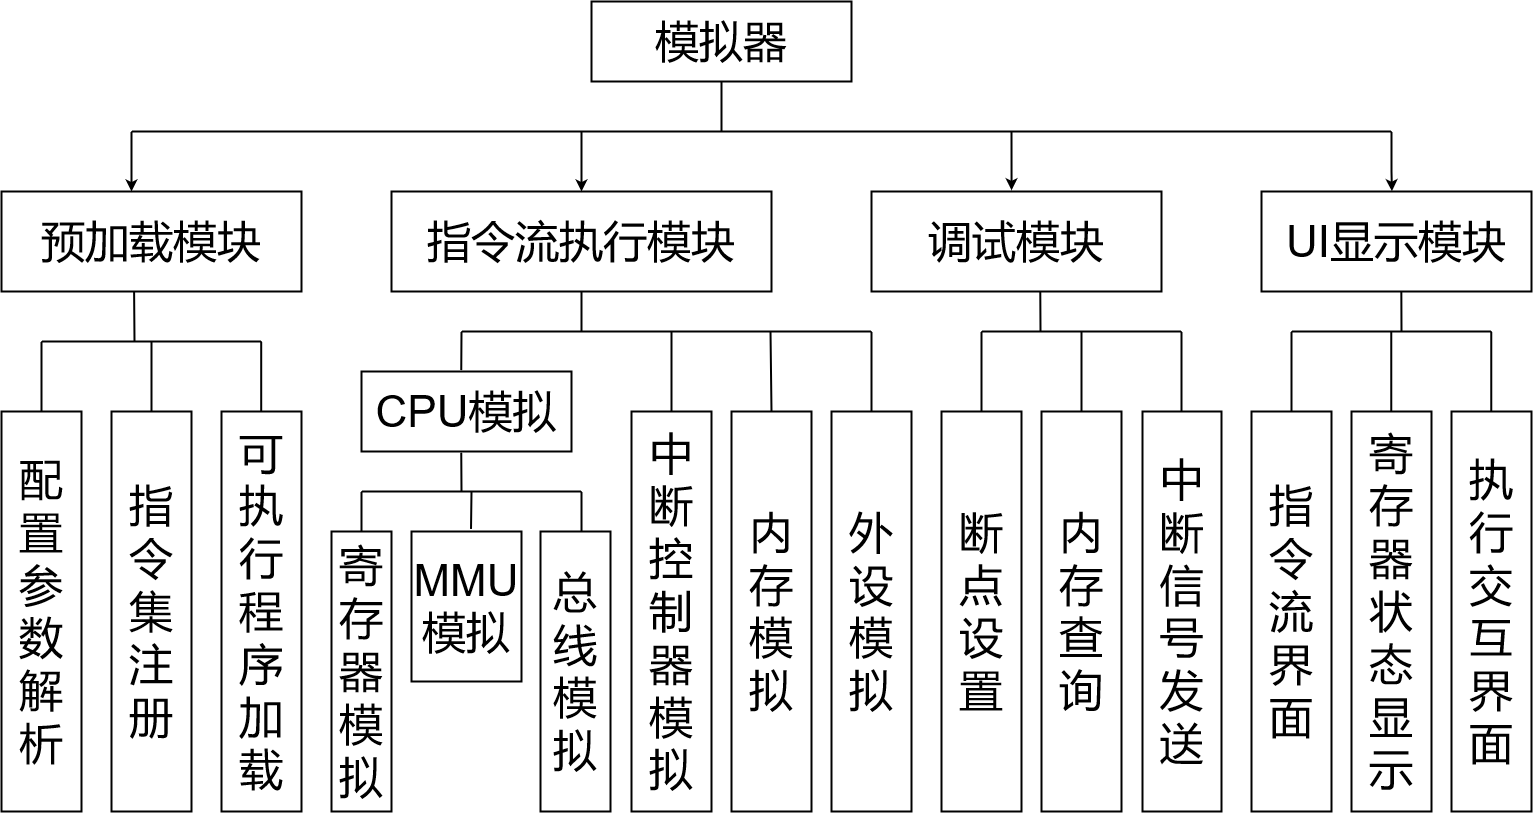
\includegraphics[width=1.0\textwidth]{sim-general.png}
  \caption{模拟器整体功能模块图}
  \label{fig:sim_general}
\end{figure}


指令流执行模块是模拟器的主体功能模块,该模块模拟了单条指令执行过程的硬件行为,包括寄存器,总线,内存,MMU,缓存,通过内存映射的I/O设备等。
\begin{figure}[h]
  \centering
  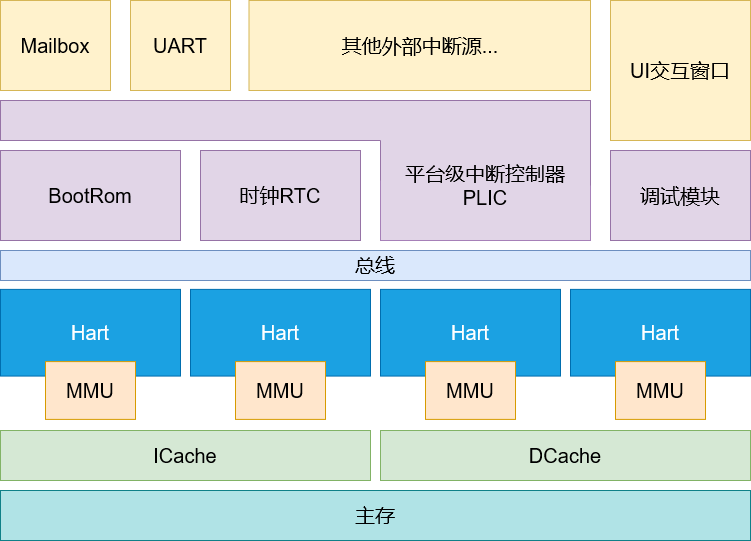
\includegraphics[width=0.8\textwidth]{cpu.png}
  \caption{处理器结构图}
  \label{fig:cpu}
\end{figure}

模拟出的RISC-V CPU整体架构如图\ref{fig:cpu}所示,每个处理器都有独立的寄存器组,内存管理单元,所
有处理器共享同一个ICache,dCache,紧随其后的是L2Cache和主
存。处理器通过总线和其他内存映射的I/O设备通信,包括BootRom,RTC,UART,PLIC,Mailbox,Debug Module.


\section{系统动态结构}
本模拟器是trace-accurate的指令集模拟器(功能模拟器),模拟器运行的基本结构如图1.1所示。


首先使用RISC-V交叉编译工具链将目标程序编译为RISC-V架构的ELF文件,然后模拟器解析该elf文件,将对
应的指令流搬运到bootrom,模拟器在配置启动后为处理器注册指令集,绑定解码器,逐条进行译码,执行。指
令译码器完成包括操作数在内的指令信息提取,找到该条指令注册时对应的功能函数,执行该功能函数,然后将
更新后的寄存器状态信息,内存状态信息同步到前端UI显示模块。在模拟器运行的过程中,用户还可以通过前端
交互调试窗口来切换模拟器运行模式,设置断点触发条件,进行单步调试,状态查询等操作。

\subsection{解码器与指令集功能函数}
RISC-V指令集是模块化的,它的核心是一个名为RV32I的基础ISA,可选的标准扩展包括MAFDC,根据应用程序
的需要,硬件可以包含或不包含这些扩展。本模拟器实现了特权指令集1.9版本,和用户指令集2.1版本的标准
拓展指令集共196条指令
的模拟。模拟器预加载时通过解析配置参数选择相应的指令集模块进行注册,并初始化解码器,流程如图1.1所示。



\subsection{指令流程控制}
指令的执行,分为取指、译码、执行三个步骤。对于单条指令,在逻辑上这三个步骤是顺序的,同步的。所以
对于功能模拟器,仍然可以把实际的流水线设计看作是单周期的CPU。

\subsection{中断控制器}

\subsection{交互调试模块}